\documentclass[11pt]{article}
\usepackage[utf8]{inputenc}
\usepackage[brazilian]{babel}
\usepackage{graphicx}
\usepackage[a4paper, top={.4in}, bottom={.65in}]{geometry}
\usepackage{subfig}
\usepackage{makecell}
\usepackage{textcomp}
\usepackage{gensymb}
\usepackage{tikz}
\usepackage{amsmath}
\usepackage{amssymb}

\begin{document}

\begin{center}
  \textbf{Experimento 07 -- PSI-3212} \\
  Natanael Magalhães Cardoso, nUSP: 8914122
\end{center}

\vspace{1.8cm}

\subsection*{Item 1.1}

\begin{figure}[h!]
  \centering
  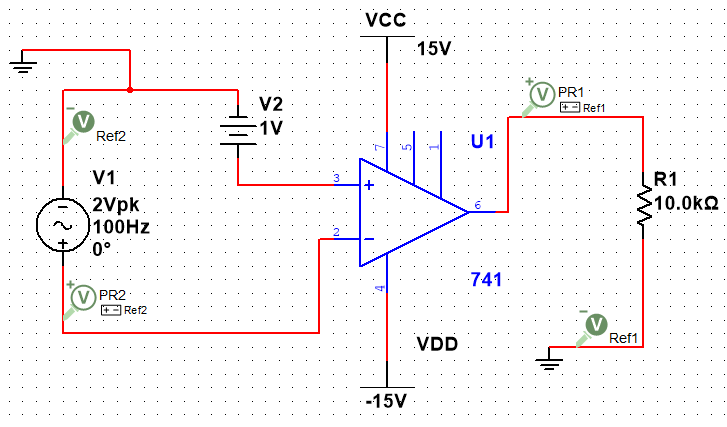
\includegraphics[width=.8\textwidth]{fig/circ1}
  \caption{Esquema do circuto}
  \label{fig:1-1-circ}
\end{figure}

\begin{figure}[h!]
  \centering
  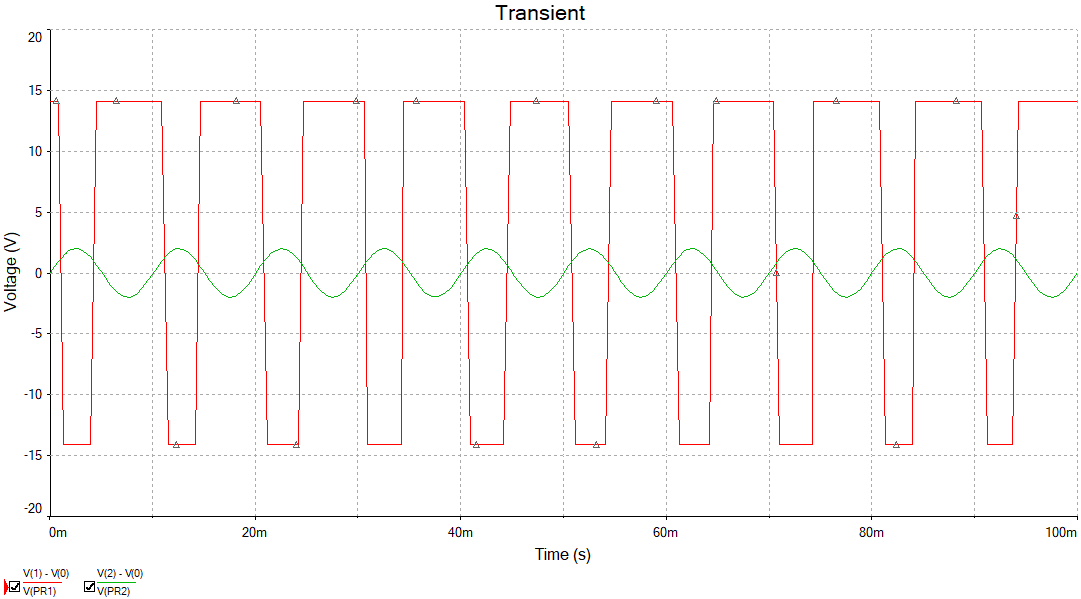
\includegraphics[width=\textwidth]{fig/sim1}
  \caption{Resultado da simulação. Em vermelho a ponta de prova PR1 ($v_{o}$) e em verde a ponta de prova PR2 ($e_{g}$).}
  \label{fig:1-1-sim}
\end{figure}

\pagebreak

\subsection*{Item 1.2}

O gráfico da figura \ref{fig:1-2} inclui a tensão de $V_{DC}$, em azul. Pela observação do gráfico, dá para ver que a curva $v_{o}$ apresenta dois extremos, que são os pontos de saturação. Além disso, observa-se que os máximos e mínimos da tensão de saída são referentes à diferença entre as tensões  $e_{g}$ e $V_{DC}$. Para valores de $e_{g} > V_{DC}$ a tensão $v_{o}$ atinge o nível de saturação inferior $V_{-SAT}$ e para valores de $e_{g} < V_{DC}$ a tensão $v_{o}$ atinge o nível superior $V_{+SAT}$. Por isso que a onda é quadrada e não senoidal. É notado também que a saturação máxima e mínima do sinal de $v_{o}$ pode ser invertida com a inversão dos sinais de entrada nos pinos 2 e 3 no OpAmp 741.

\begin{figure}[h!]
  \centering
  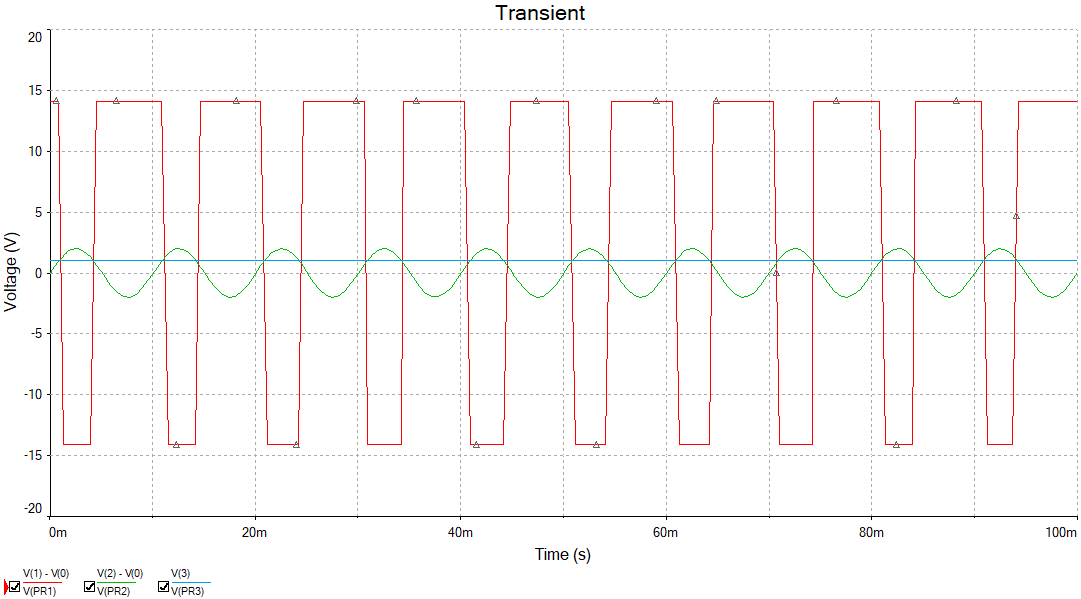
\includegraphics[width=\textwidth]{fig/sim1_vdc}
  \caption{Simulação do circuito da figura \ref{fig:1-1-circ} com a tensão $V_{DC}$ em azul.}
  \label{fig:1-2}
\end{figure}

\subsection*{Item 1.3}

\begin{figure}[h!]
  \centering
  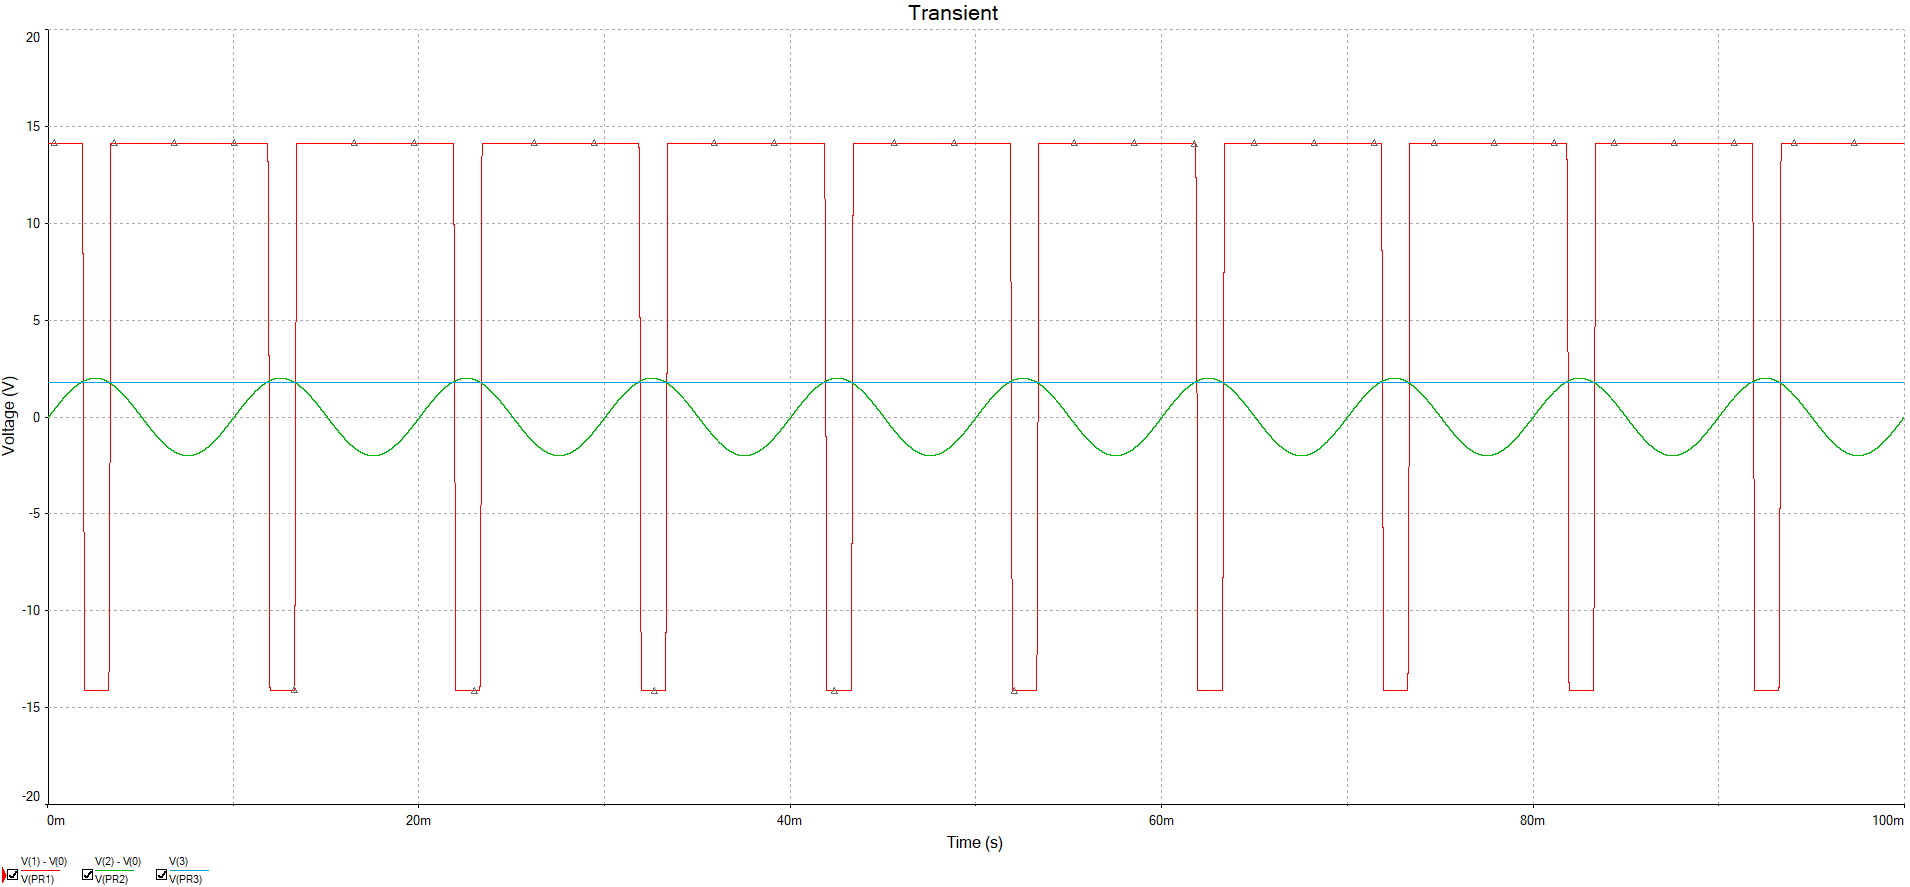
\includegraphics[width=\textwidth]{fig/sim1_3}
  \caption{Simulação do circuito da figura \ref{fig:1-1-circ} para $V_{DC}$ = 1.8 V.}
  \label{fig:1-3}
\end{figure}

Foi observado que o tempo em nível alto fica menor, pois aumentando o valor de $V_{DC}$, diminiu-se o tempo em que $e_(g) > V_{DC}$.

Os valores medidos com o cursor do simulador foram:

Tempo em nível alto: 8.35 ms

Tempo em nível baixo: 1.40 ms

\subsection*{Item 1.4}

Com a simulação da figura \ref{fig:1-1-sim} observa-se que o sinal de tensão $v_{o}$ possui valores maximos ou mínimos de acordo com o sinal positivo ou negativo da curva $e_{g}$, mas este positivo e negativo não é em relação a zero. Com a simulação da figura \ref{fig:1-2}, que mostra a tensão $V_{DC}$ e o experimento da figura \ref{fig:1-3} variando o valor de $V_{DC}$, ficou claro que a tensão $V_{DC}$ define o positivo e o negativo. Nesse sentido, este circuito é um comparador porque compara dois sinais, de tal forma que $v_{o}$ é máximo quando $V_{DC} - e_{g}$ é maior que zero e mínimo caso contrário.

\subsection*{Item 2.1.a}

\begin{figure}[h!]
  \centering
  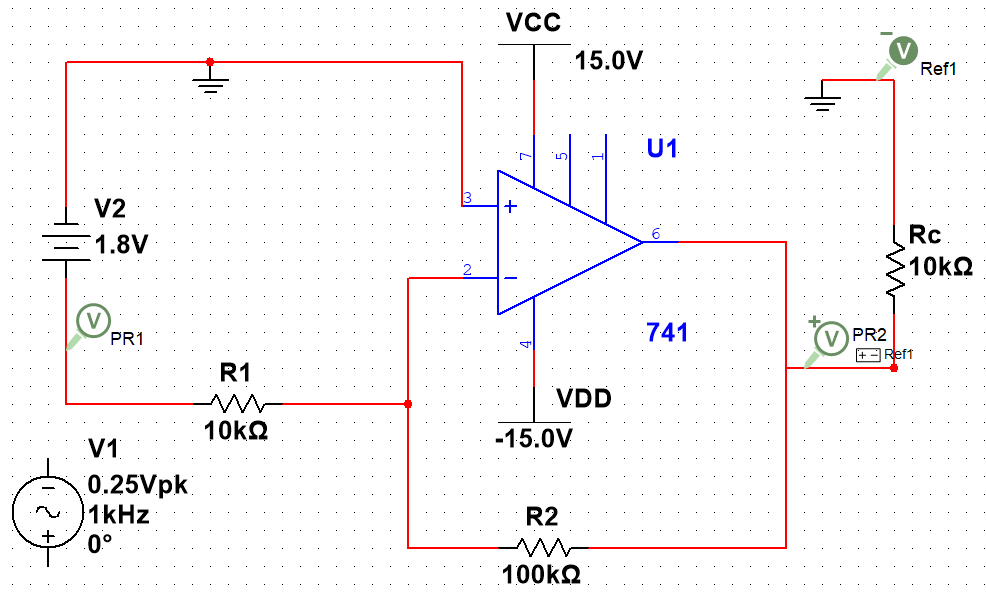
\includegraphics[width=.8\textwidth]{fig/circ2_a}
  \caption{Esquema do circuito.}
  \label{fig:circ2a}
\end{figure}

\begin{figure}[h!]
  \centering
  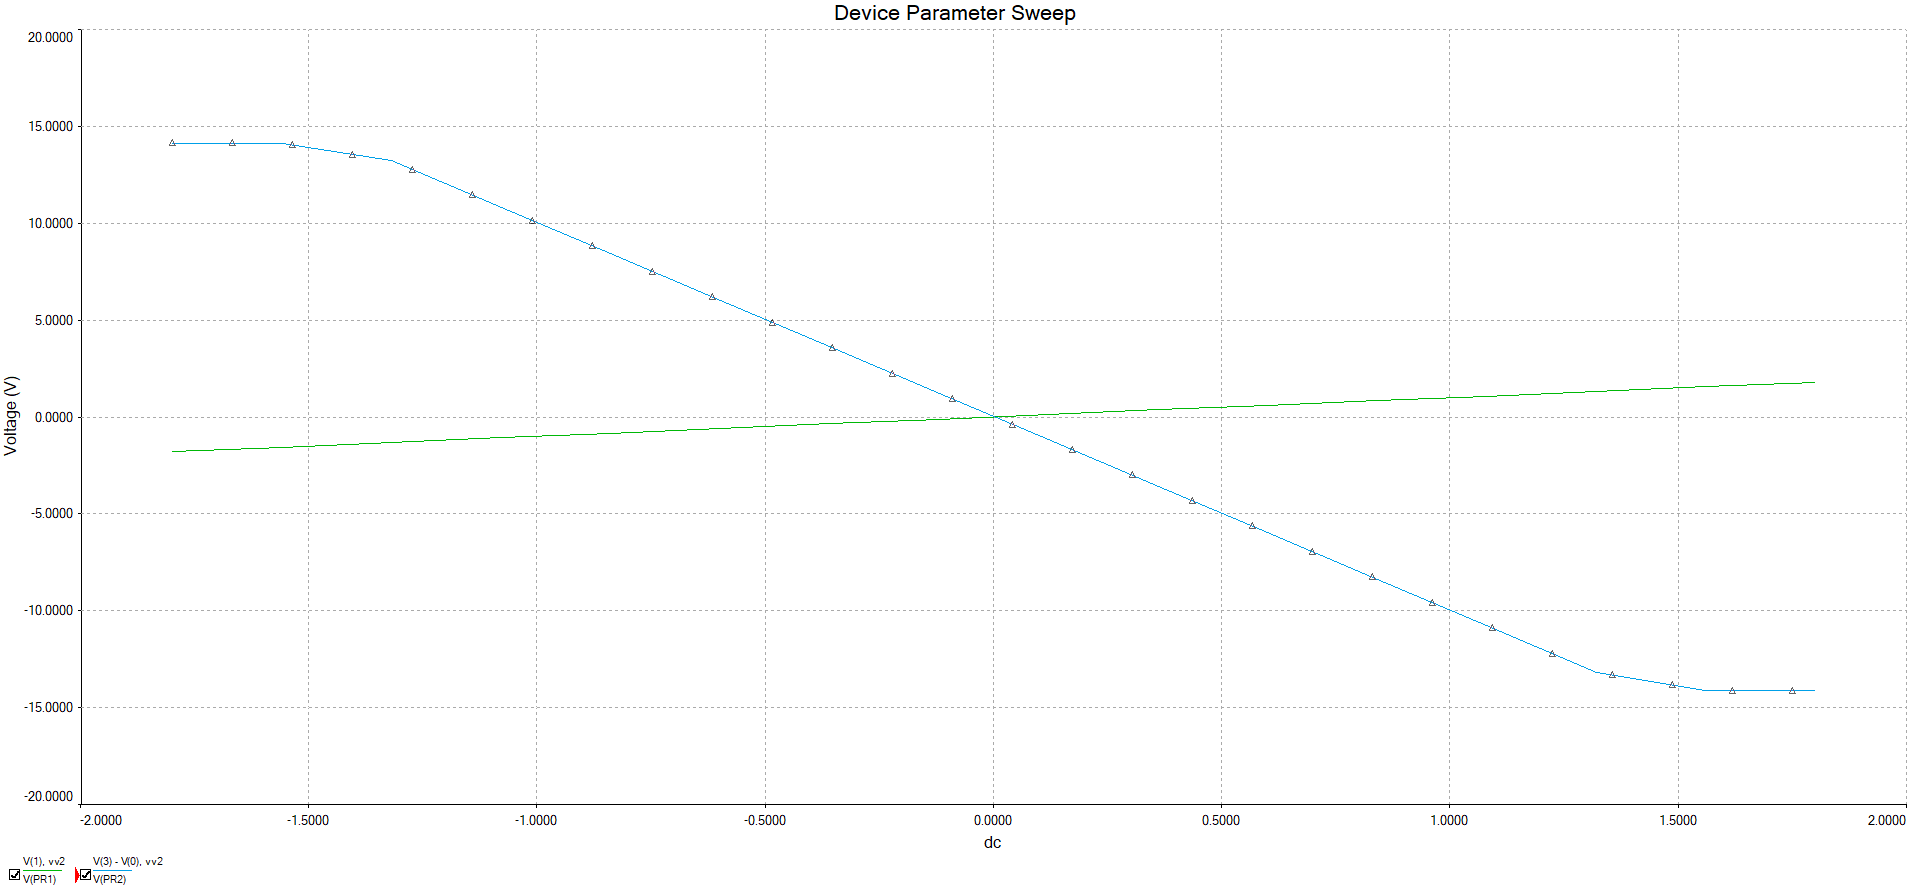
\includegraphics[width=\textwidth]{fig/sim2_a}
  \caption{Simulação do circuito da figura \ref{fig:circ2a}.}
  \label{fig:2-1a}
\end{figure}

\pagebreak

\subsection*{Item 2.1.b}

O gráfico da figura \ref{fig:circ2a}, mostra que a tensão de saída tem polaridade invertida, ou seja,  para valores positivos de tensão de entrada, a tensão de saída é negativa e vice-versa. E ainda tem  uma amplitude muito maior (em módulo), pois é um amplificador.

\subsection*{Item 2.2.a}

\begin{figure}[h!]
  \centering
  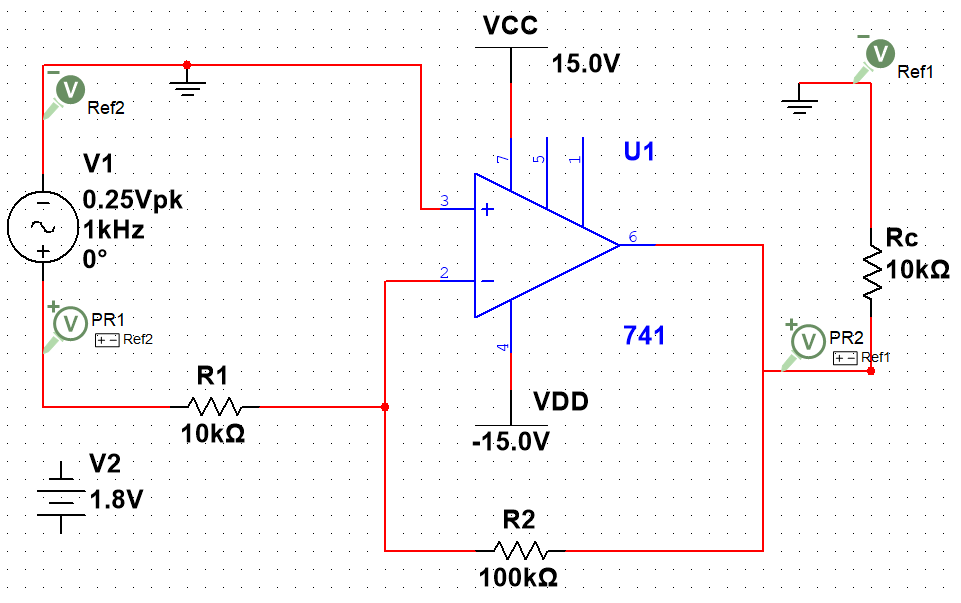
\includegraphics[width=.8\textwidth]{fig/circ2_b}
  \caption{Esquema do circuito.}
  \label{fig:circ2b}
\end{figure}

\begin{figure}[h!]
  \centering
  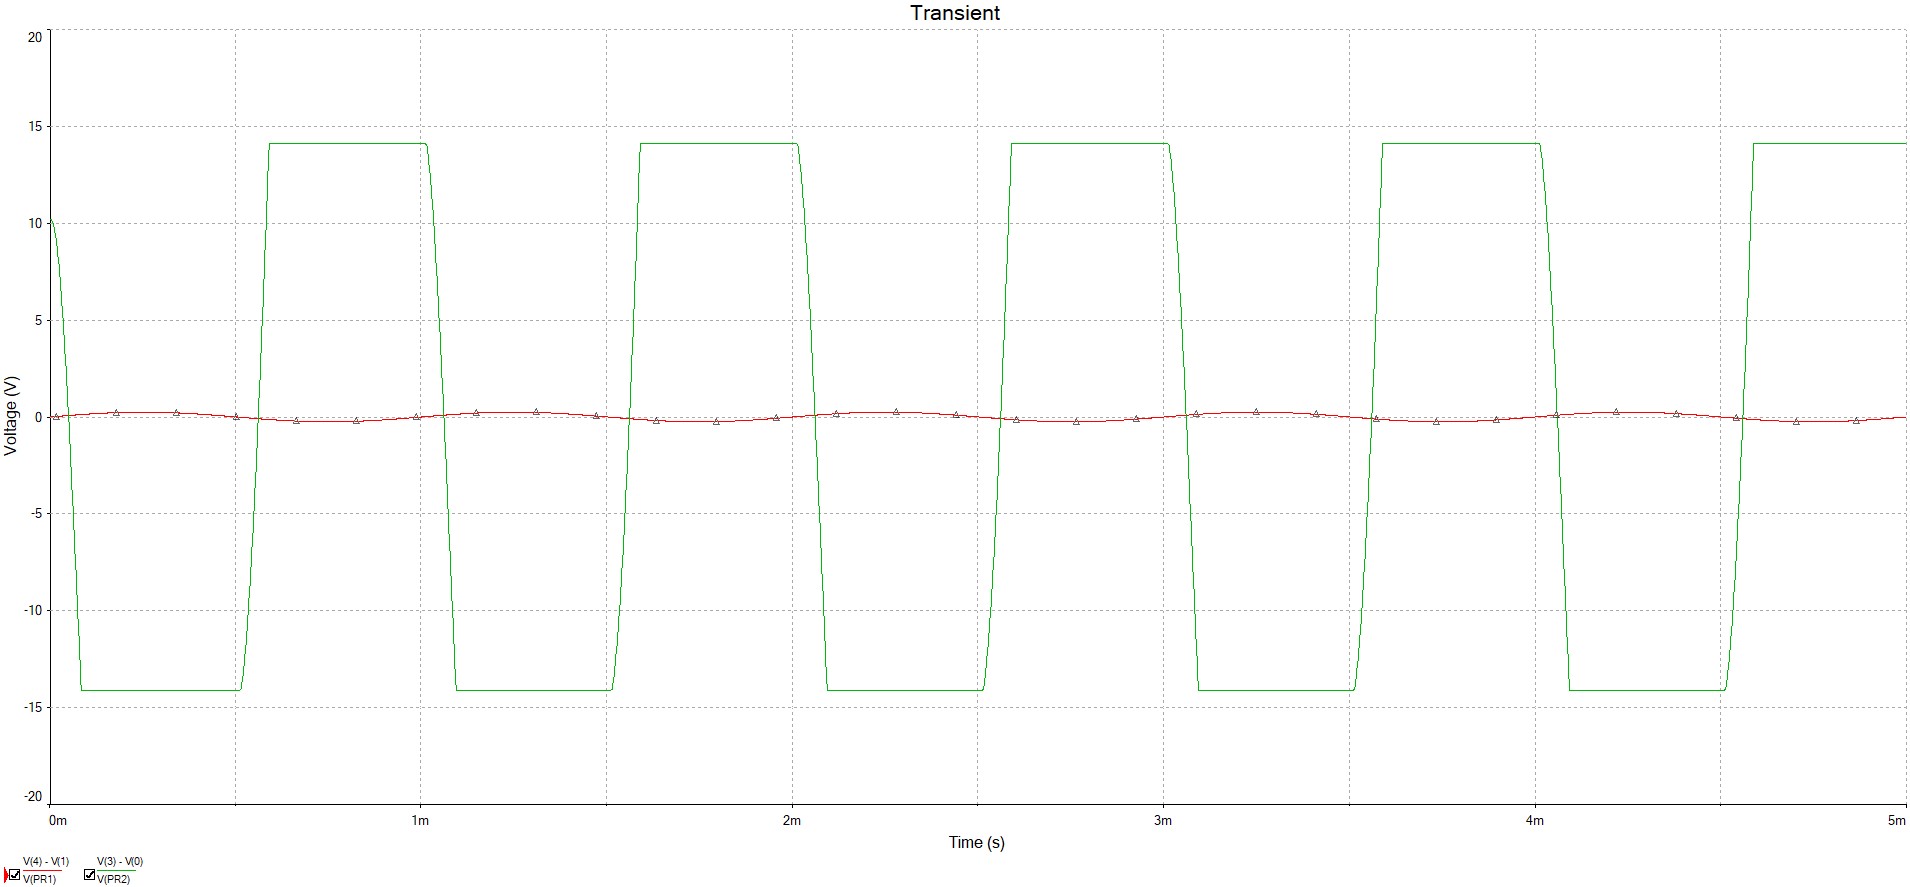
\includegraphics[width=\textwidth]{fig/sim2_b}
  \caption{Simulação do circuito da figura \ref{fig:circ2b}.}
  \label{fig:2-2b}
\end{figure}

\subsection*{Item 2.2.b}

Aqui se observa que o comportamento visto no item (2.1) também é válido para tensões AC. Diferente do item (1), a tensão de saída satura quando a tensão de entrada inverte a polaridade, já que neste circuito a entrada 3 do aplificador está aterrada.

\pagebreak

\subsection*{Item 3.a}

\begin{figure}[h!]
  \centering
  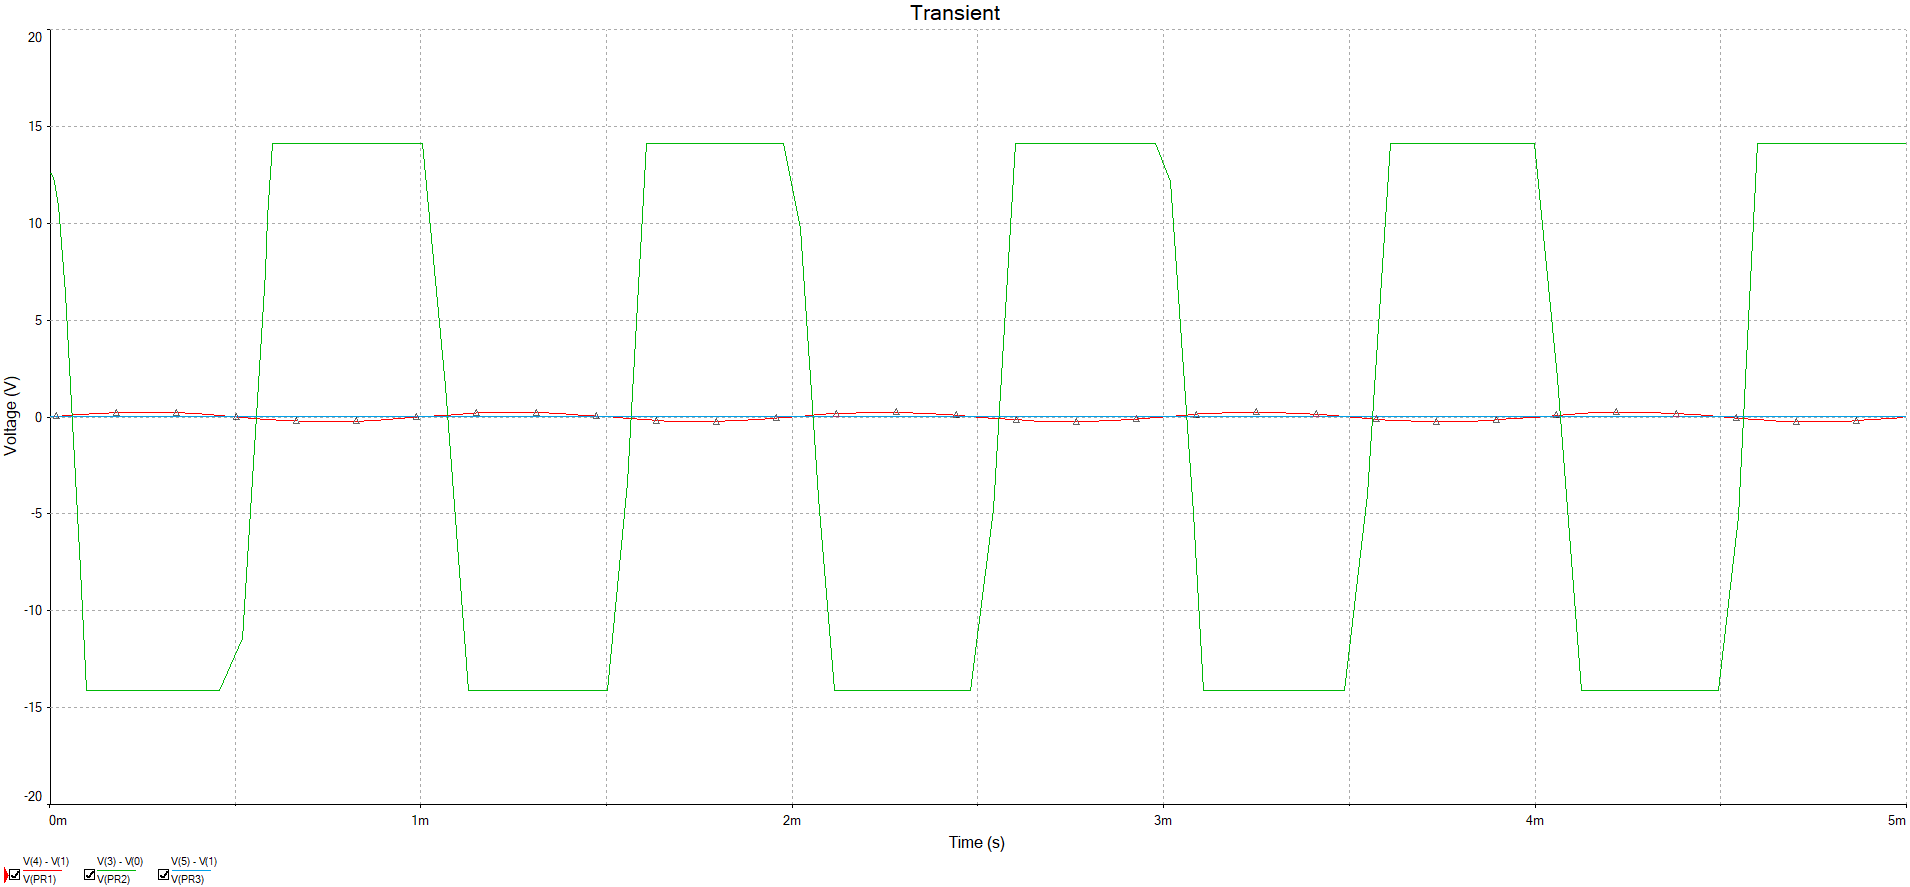
\includegraphics[width=\textwidth]{fig/sim3a}
  \caption{Simulação para $V_{DC}$ = 0 V.}
\end{figure}

\subsection*{Item 3.b}

\begin{figure}[h!]
  \centering
  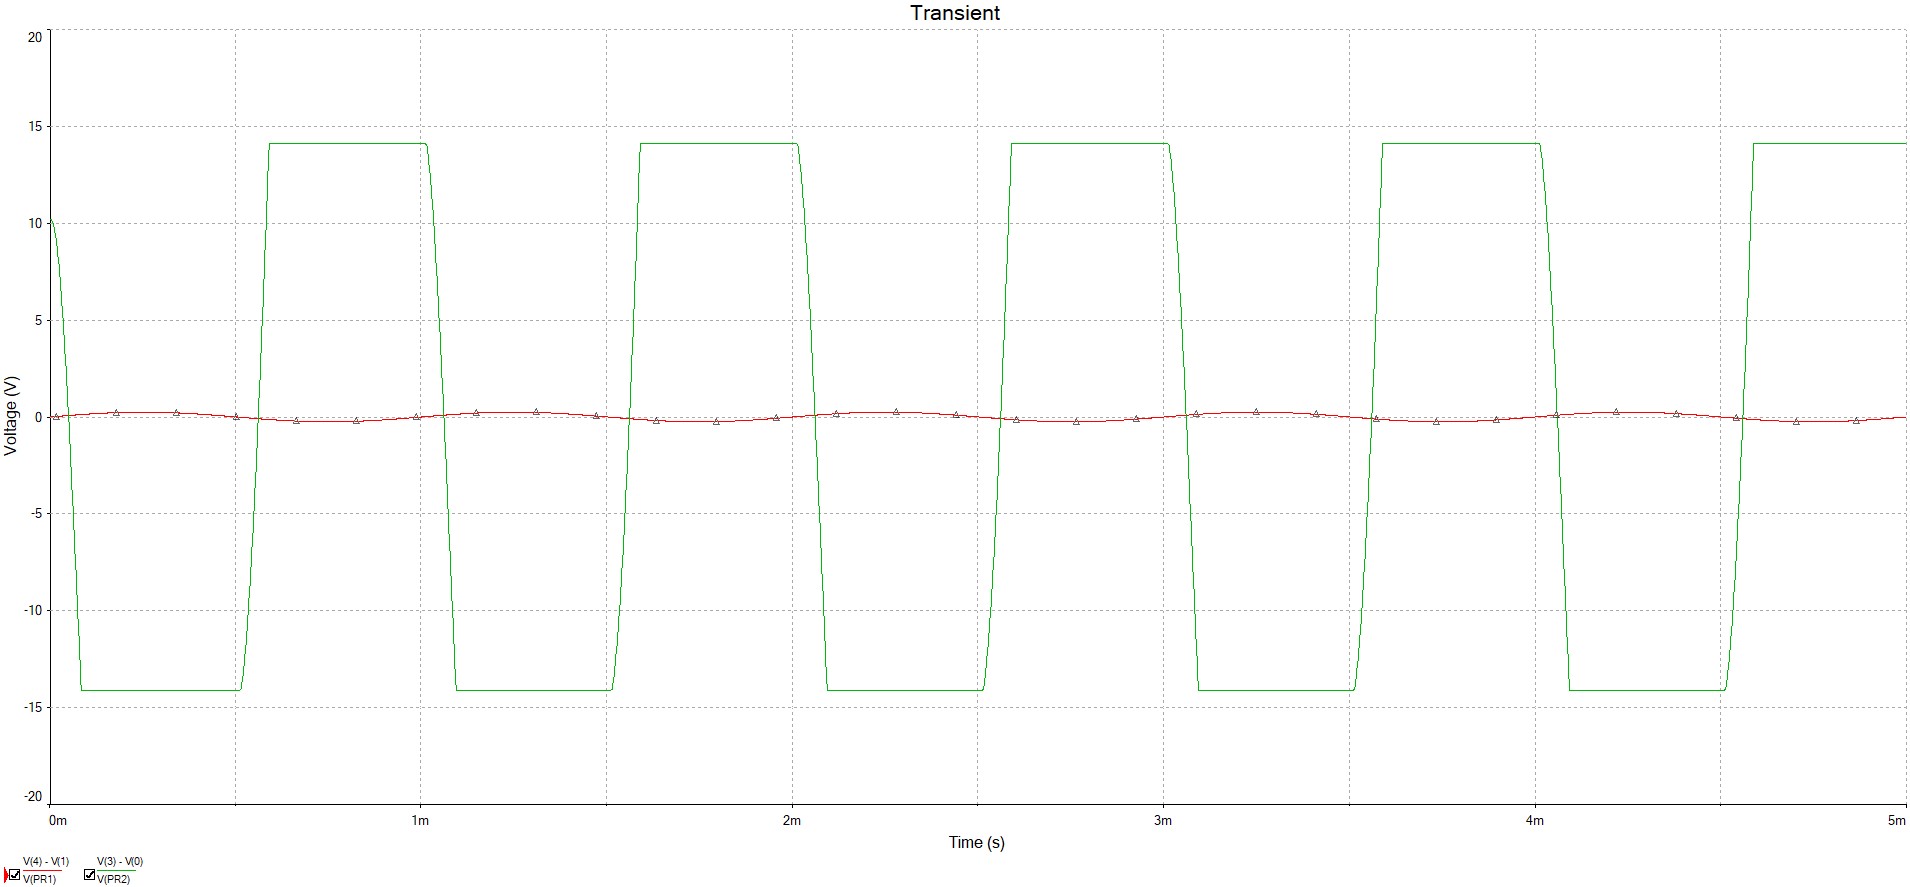
\includegraphics[width=\textwidth]{fig/sim2_b}
  \caption{Simulação para $V_{DC}$ = 1 V.}
\end{figure}

\pagebreak

\subsection*{Item 3.c}

\begin{figure}[h!]
  \centering
  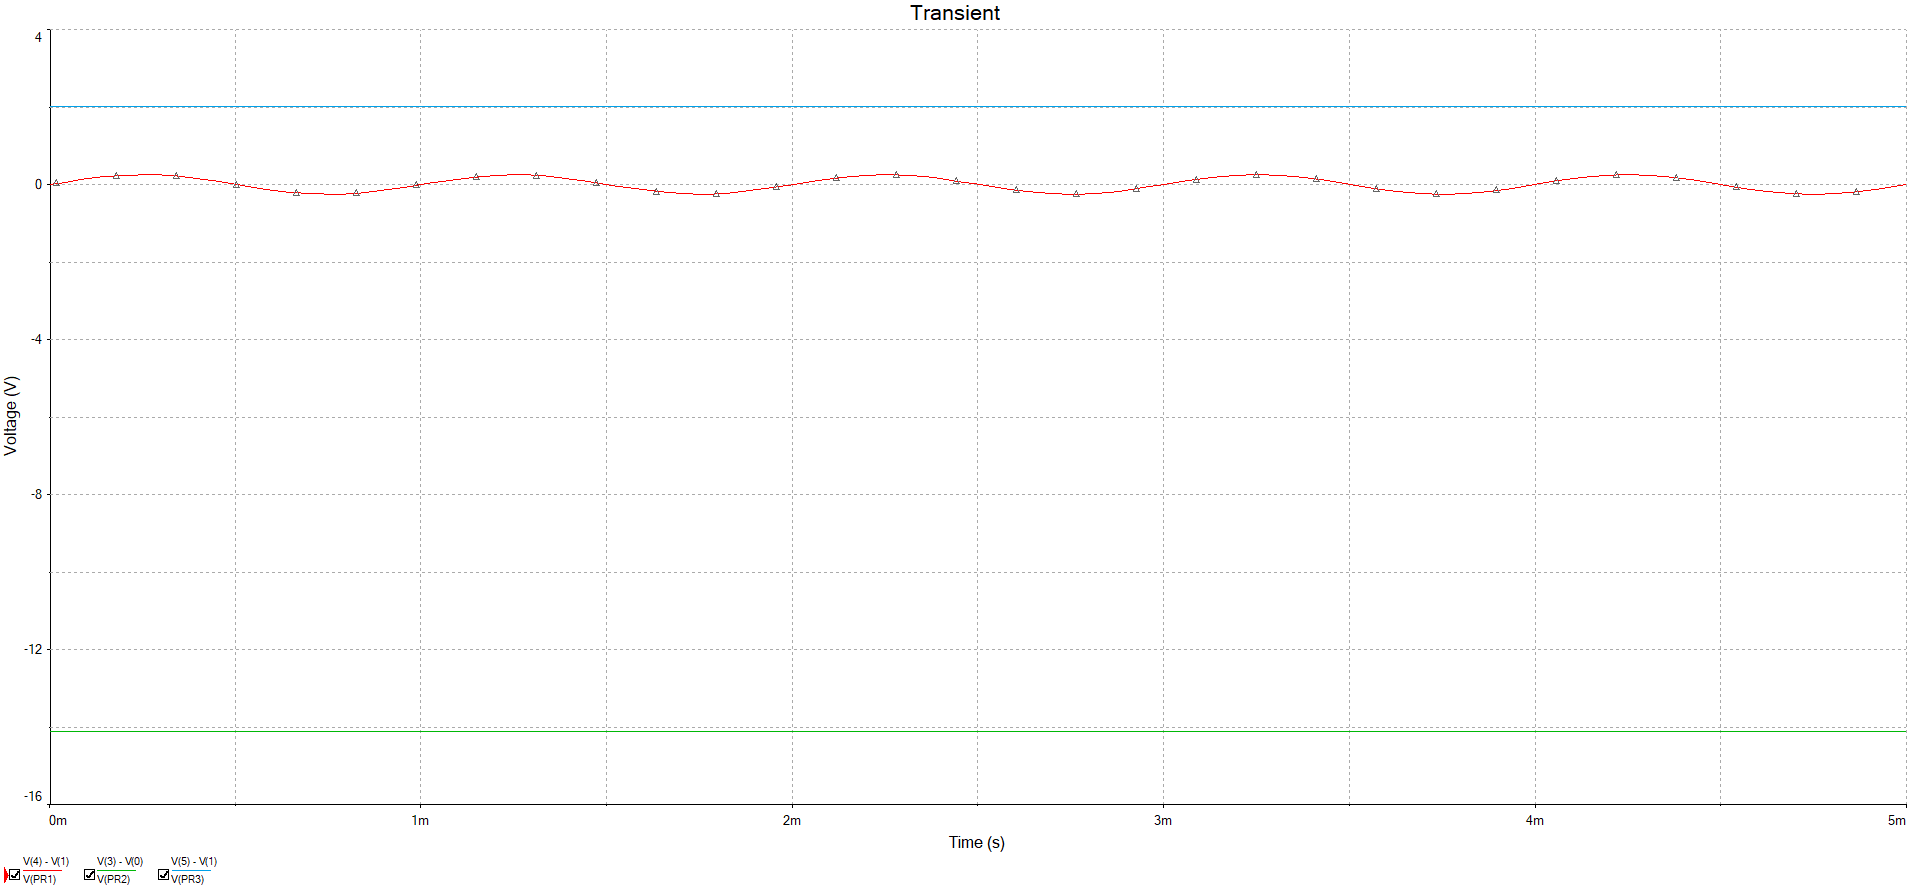
\includegraphics[width=\textwidth]{fig/sim3c}
  \caption{Simulação para $V_{DC}$ = 2 V.}
\end{figure}


\end{document}
